\chapter{Implementations} \label{ch:implementations}
\vcomment{This chapter shows how things described within the research protocol are performed. By separating it out, I can focus on things like verifying accuracy / comparisons / demos / pseudocode without cluttering up the discussion of the actual methodologies of the next chapter. That way parameters choices, etc. can be more clearly highlighted. However, this section is apt place to discuss how varying parameters influences whatever methods are being used.}


\section{Calculating the Hessian via FFT}

% assuming that we already know how the 
Efficient implementation of the Frangi filter ultimately relies on performing a 2D Gaussian blur in frequency space. Here we demonstrate that our FFT implementation of Gaussian blur is commensurate with other implementations. 

In \cref{fig:fft-gaussian-demo}, we demonstrate the compatibility of standard convolution and FFT convolve. Each row corresponds to a different scale at which Gaussian blurring  occurs. Column (a) is standard convolution with a sampled Gaussian kernel, column (b) is FFT-convolution with a Gaussian kernel, and column (c) is a FFT-convolution with the ``discrete Gaussian kernel''. In column (d), the 1D discrete Gaussian kernel (in green) is plotted against the sampled continuous Gaussian kernel (in black). Note that each of the images in the first three columns are scaled the same.
\begin{figure}
  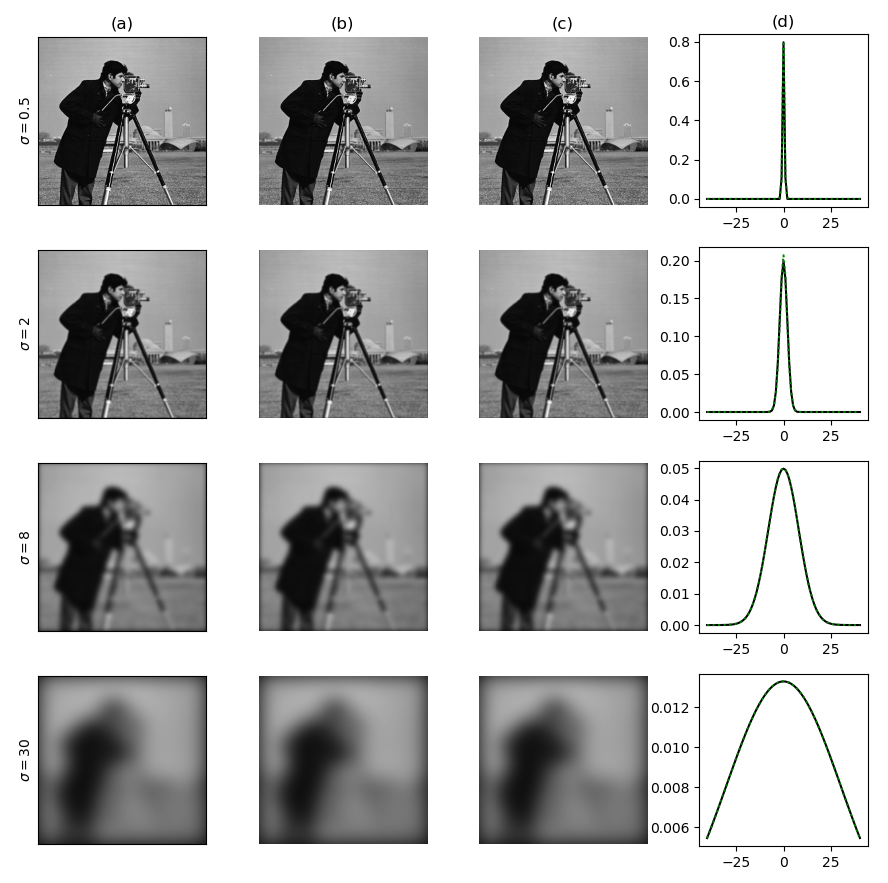
\includegraphics[width=\linewidth]{fft_gaussian_demo}
  \caption{Compatibility of Gaussian convolution strategies}
  \label{fig:fft-gaussian-demo}
\end{figure}

In \cref{fig:semigroup-demo}, we show these same three methods of Gaussian blur but for a large scale
($\sigma=45$). For each method of taking the Gaussian blur ((a) - standard convolution with sampled kernel, (b) fft with sampled kernel, (c) fft with discrete kernel), the top row is one round of Gaussian blur with $\sigma=45$ and the bottom row is two progressive passes of Gaussian blur ($\sigma_1 = 10, \sigma_2 = 35$). The mean squared error and mean absolute error between the one-pass and two-pass versions are outputted below. Code for this demo can be found in \texttt{hfft.semigroup\_demo}.
The discrete kernel performs very slightly better than the sampled versions. We originally attempted
this demonstration with a much larger sigma (say $\sigma=150$) and multiple iterations, but unfortunately multiple passes cause the ``noise'' from zeroing out around the boundaries to become very noticable after several iterations (here, we've opted to crop out a radius of pixels from around the edges equal to the standard deviation of the Gaussian before we calculated the MAE or MSE). We could show this again with a zero border or maybe even just a 1D signal.

\begin{table}
  \centering
  \begin{tabular}{c|cc}
   blurring method   & MSE & MAE \\
    \hline
spatial convolution, sampled kernel & 0.00054426 & 0.02015643 \\
FFT convolution, sampled kernel & 0.00055205 & 0.02029916 \\
FFT convolution, discrete kernel & 0.00054406 & 0.02015336
    \end{tabular}
\end{table}


\begin{figure}
  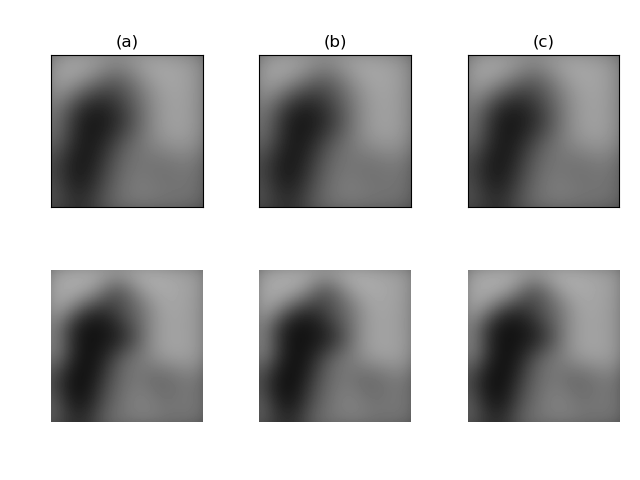
\includegraphics[width=\linewidth]{semigroup_demo}
  \caption{Iterative Gaussian blur}
  \label{fig:semigroup-demo}
\end{figure}

We further confirm the commensurate nature of Gaussian blur techniques by comparing the three techniques on a placental image and using each to calculate Frangi targets. The code can be found in \texttt{hfft\_accuracy.py}. In \cref{tab:mse-G-sigma-0.3}, \cref{tab:mse-F-sigma-0.3}, \cref{tab:mse-G-sigma-5} and \cref{tab:mse-F-sigma-5} we compare the mean squared error of a single image blurred (A) with standard spatial convolution, (B) with FFT sampled Gaussian kernel, and (C) with the discrete kernel. We see that the standard convolution and discrete convolution are very similar, while the sampled discrete Gaussian is off by two orders of magnitude, but still reasonably small. We further confirm these by viewing the intensity of the images and the Frangi targets themselves across an arbitrarily chosen horizontal cross section of the image. As seen in \cref{fig:cross-sec-G-sigma=0.3}, \cref{fig:cross-sec-F-sigma=0.3},
\cref{fig:cross-sec-G-sigma=5}, \cref{fig:cross-sec-F-sigma=5}, the peaks of the Gaussian blurred image all still occur at the same places, as do the Frangi responses. We repeated this procedure up to $\sigma=90$ and found a situation similar to $\sigma=5$; it was only in very small scales where there was any noticeable difference at all.


\begin{table}
  \parbox{.45\linewidth}{
  \centering
  \begin{tabular}{c|ccc}
    &  A & B & C \\
    \hline
  A & -  & 1.296e-03 & 6.772e-06 \\
  B & -  & - & 1.247e-03 \\
  C & -  &  - &  - \\
  \end{tabular}
\caption{MSE of Gaussian blurs of an image ($\sigma=0.3$)}
\label{tab:mse-G-sigma-0.3}
}
    \parbox{.45\linewidth}{
  \centering
  \begin{tabular}{c|ccc}
      &  A &  B         & C \\
      \hline
    A &  - &  4.256e-06 & 5.537e-08 \\
    B &  - &  -         & 4.337e-06 \\
    C &  - &  -         &  - \\
  \end{tabular}
  \caption{MSE of Frangi scores $\sigma=0.3$}
  \label{tab:mse-F-sigma-0.3}
}
  \end{table}



\begin{figure}
  \centering
  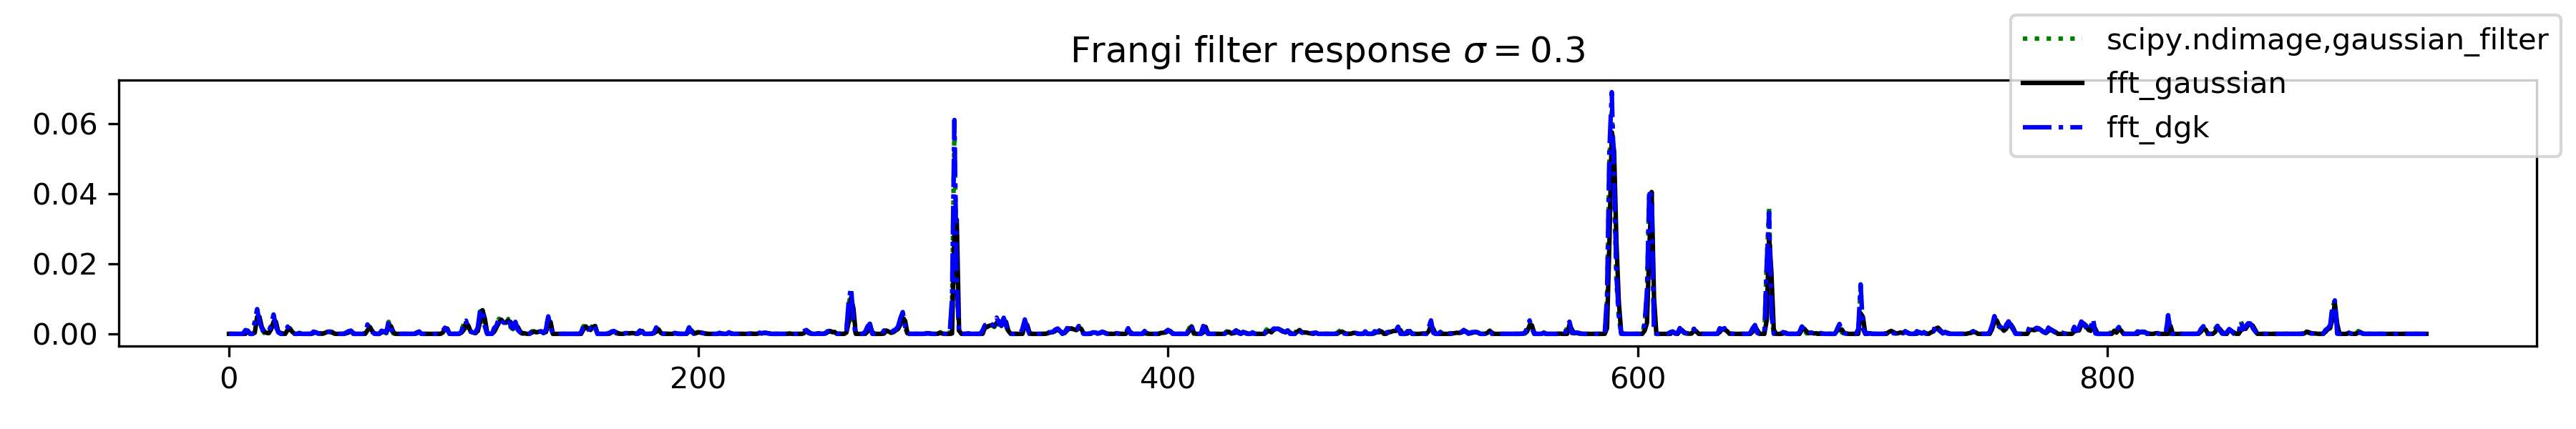
\includegraphics[width=\linewidth]{Fslice_sigma=3}
  \caption{Image cross-section of Gaussian blurred images}
  \label{fig:cross-sec-G-sigma=0.3}
\end{figure}

\begin{figure}
  \centering
  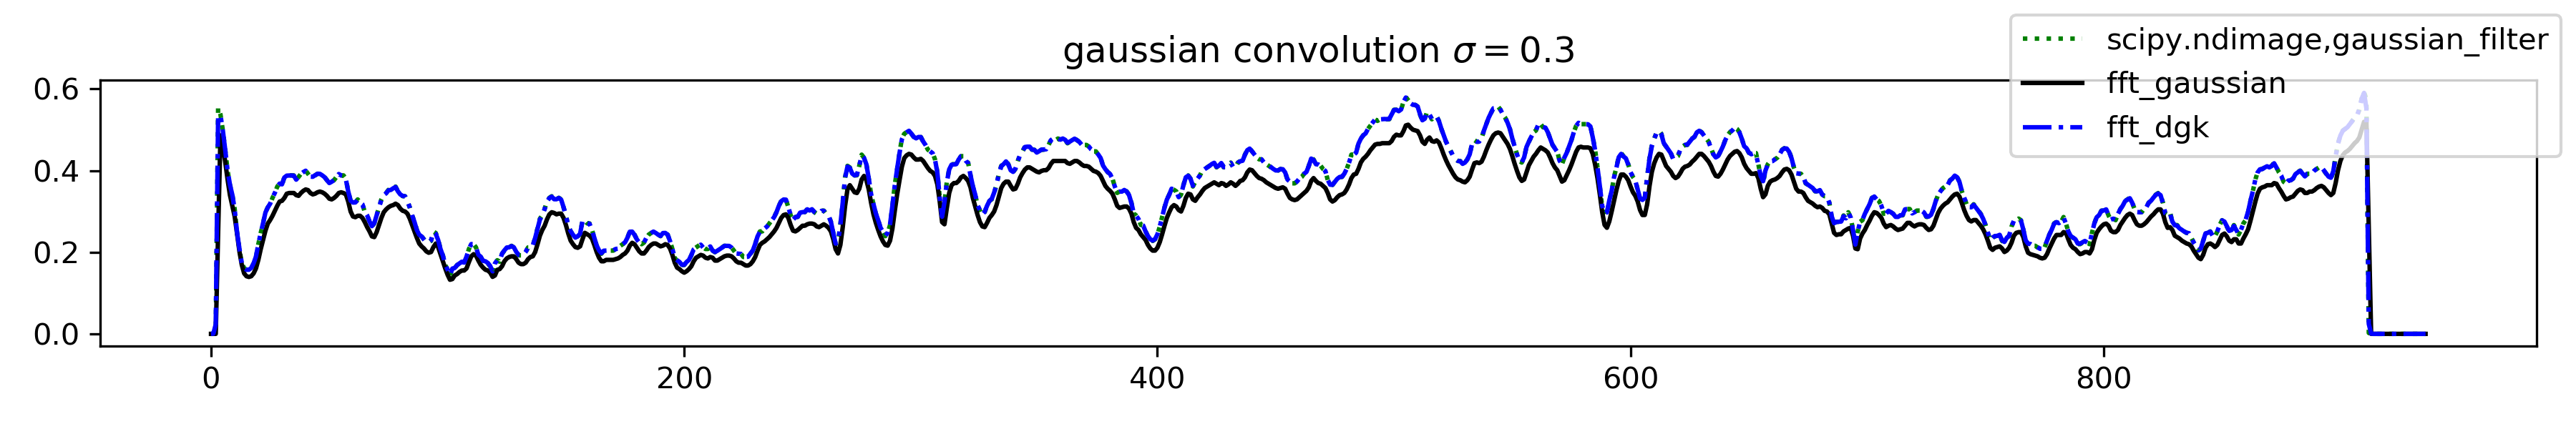
\includegraphics[width=\linewidth]{Gslice_sigma=3}
    \caption{Image cross-section of Frangi targets images}
    \label{fig:cross-sec-F-sigma=0.3}
\end{figure}



\begin{table}
  \parbox{.45\linewidth}{
    \centering
    \begin{tabular}{c|ccc}
      &  A & B & C \\
      \hline
      A & -  &  9.012e-06 & 8.629e-09 \\
      B & -  & - & 9.031e-06 \\
      C & -  &  - &  - \\
    \end{tabular}
    \caption{MSE of Gaussian blurs of an image ($\sigma=5$)}
    \label{tab:mse-G-sigma-5}
  }
  \parbox{.45\linewidth}{
    \centering
    \begin{tabular}{c|ccc}
      &  A &  B         & C \\
      \hline
      A &  - &  9.388e-05 8.383e-07 \\
      B &  - &  -         & 9.599e-05 \\
      C &  - &  -         &  - \\
    \end{tabular}
    \caption{MSE of Frangi scores $\sigma=5$}
    \label{tab:mse-F-sigma-5}
  }
\end{table}

\begin{figure}
  \centering
  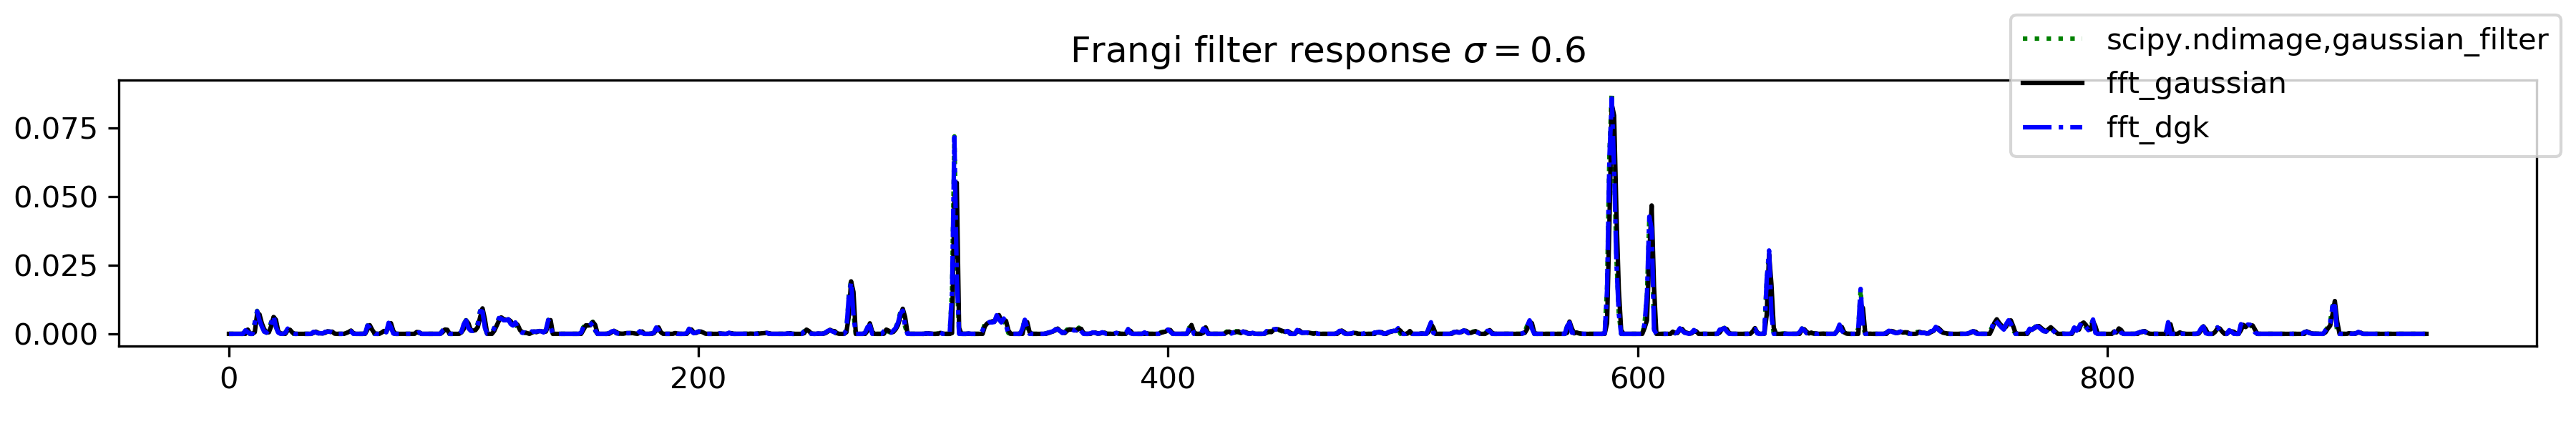
\includegraphics[width=\linewidth]{Fslice_sigma=6}
  \caption{Image cross-section of Gaussian blurred images $\sigma=5$}
  \label{fig:cross-sec-G-sigma=5}
\end{figure}

\begin{figure}
  \centering
  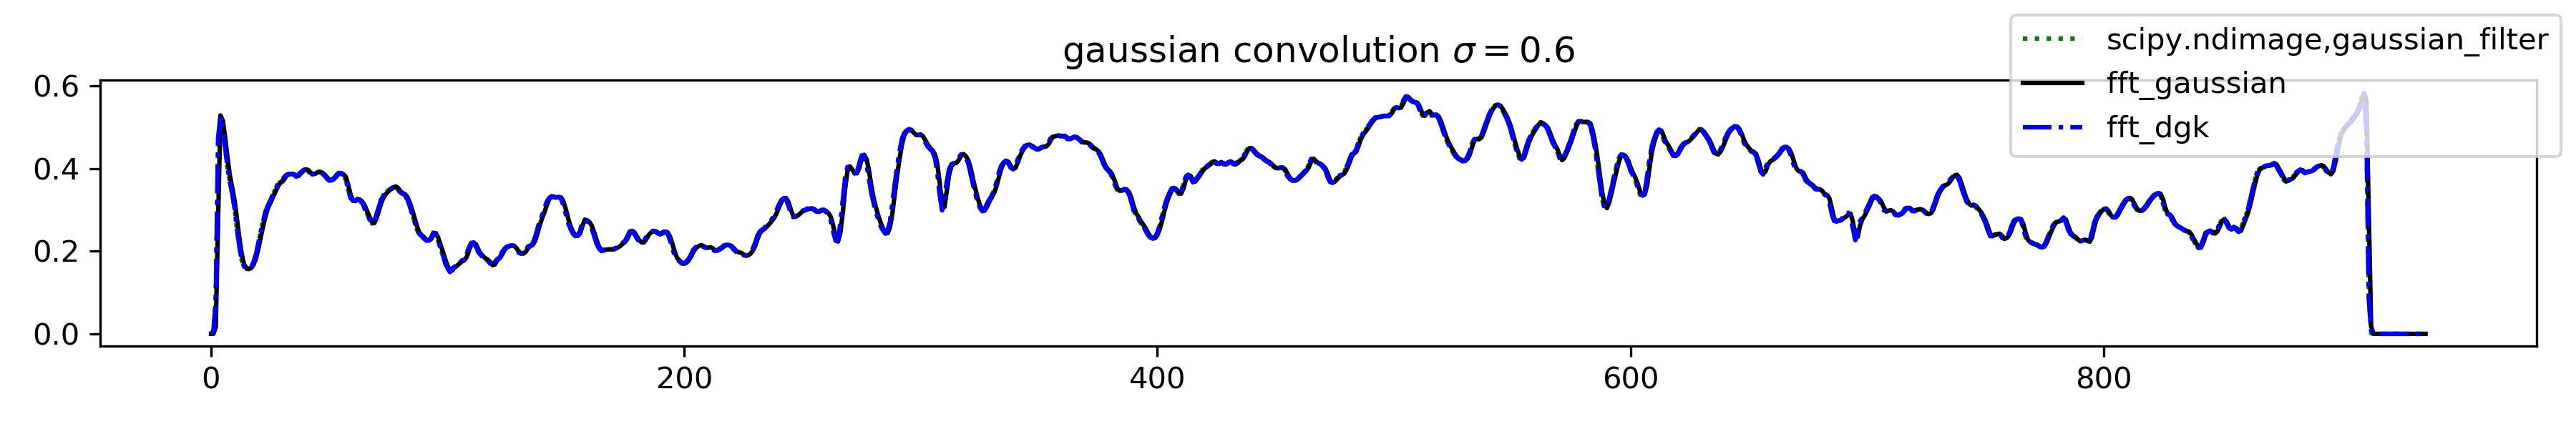
\includegraphics[width=\linewidth]{Gslice_sigma=6}
  \caption{Image cross-section of Frangi targets images $\sigma=5$}
  \label{fig:cross-sec-F-sigma=5}
\end{figure}


Finally, we wish to demonstrate the point of this comparison--that $FFT-based$ convolution is much faster than spatial convolution. We took a much larger sample ($2200 \times 2561$) and timed each method of convolution (average of three trials) for a large number of samples: logarithmic between $\sigma=1$ and $\sigma=128$ with 32 steps. The result shows that the convolution time seems to at least linearly increase with the size of the kernel, whereas FFT is independent of choice of scale.

\begin{figure}
  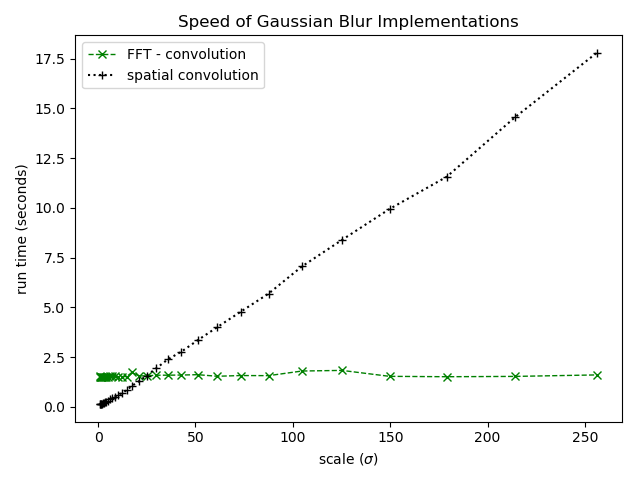
\includegraphics[width=\linewidth]{convolution-runtime-demo}
  \caption{Time required}
\end{figure}

\section{Postprocessing Techniques}
We display several four relatively immediate postprocessing techniques on the multiscale Frangi output to obtain an actual PCSVN extraction. Again we stress that the Frangi filter itself does not produce a segmentation, but instead could be used as a preprocessing step. In fact, Frangi in his original paper \cite{frangi-paper} refrained from any explicit analysis of the Frangi score apart from taking the maximum across all scales, as in \cref{frangi-vesselness-max}. Still, we wish to demonstrate some several immediate methods of postprocessing these samples in order to illustrate the usefulness of this optimized Frangi filter. 

Unfortunately, even with our ``rescaled'' Frangi filter, this $\alpha$ cannot be picked without regard for the particular image domain. Equally problematic, we cannot guarantee that the Frangi filter will decay as our scale exceeds the the bounds where structure is expected to be found. Ideally we could create a filter that would do that.

\subsection{Method A: Fixed Threshold}

In the fixed threshold method, we say that a pixel $(x,y)$ of the image corresponds to a vessel if
$V_{\max} >  \alpha$. This $\alpha$, as noted above, is unfortunately highly dependent on the image domain, and this merging method will tend to happily allow noise generated from scales that are too large or too small. \vtodo{PUT A FIGURE HERE OF BIG BLOTCHES WHEN THE SCALE IS TOO LARGE}. Another issue with this is the individual scales of the Frangi filter in the extreme cases are not known to scale--although Lindeberg introduced a normalization factor based on the scale to apply to the derivatives, we do not know of an optimal factor to use.


\subsection{Method B: Percentile Based Merging}

The idea behind percentile-based merging is beneficial for large multiscale methods. At each scale, we would like to assume that there is \textit{some} curvilinear content that could be identified. With that in mind, we could simply accept from each scales scores in a very high percentile. We chose for our demonstration a fairly large percentile, $95$, and furthermore boster this by requiring that any selected pixels be in the 95th percentile of nonzero and unmasked pixels--otherwise the average is artificially low due to the large background and pixels with zero Frangi score. The use of percentiles removes dependence of picking a particular threshold on the problem, while allowing the most prominent features to emerge at each scale, but of course it unfortunately treats all scales equally, so the success of the multiscale approach here is very dependent on choice of $\sigma_{\min}$ and $\sigma_{\max}$.

\subsection{Method C: Scale-Based Random Walker}

We observed that areas where Frangi scores are zero in well-behaved samples seem to neatly outline prominent vascular features. Following this idea, we employed a random walker segmentation \cite{Grady-Random-Walks} (which is implemented by \texttt{scikit-image}). Random walk segmentation comes about by solving a diffusion problem over a discrete array (in this case, the Frangi vesselness score itself) given starting markers. At each scale, we positively labeled pixels whose Frangi score was very high ($V_\sigma(x_0,y_0) > .4$), and negatively labeled pixels whose score was $0$ (i.e. where the leading principal eigenvalue was positive). The result of this technique is demonstrated in \cref{rw_demo-scalewise} and the result (along with the original sample for comparison) is shown in \cref{fig:rw-demo-merged}.
In \cref{rw-demo-scalewise}, the first column is the Frangi vesselness score at that scale, where black is a score of 0, to emphasize the difference between a score of zero and even a very small positive score, which appear in blue. The middle score are markers passed to the random walker--blue are seeds labelled with a ``1'' (where the Frangi vesselness score is 0), green is labeled ``2'' (where V > .4), and purple represents unknowns that will either assigned either label. In the last column, the result of the random walker is given--areas that have been added to the label ``2'' are shown in yellow. Although the result of random walker segmentation is technically a binary matrix, we still show the original seeds of label 2 in green for easier comparison. Similarly, the purple in the right column has actually been labeled ``1'' for non-vascular, but is left in its original color to emphasize what was assigned background. In \cref{fig:rw-demo-merged} we show the original image and the result of merging all positively marked pixels at each scale. Black means the pixel was unmatched, while increasing colors of blue (larger scales) to white (smaller scales) indicate the smallest scale from which a pixel was marked after the random walker technique. \vtodo{Do I need to over this in math methods section?} Though we shall set up the multiscale method slightly differently in \cref{ch:results-analysis}, we used a Frangi anisotropy coefficient of $\beta=0.35$ , and 12 scales logarithmically spaced from $\sigma_1 = 2^{-1.5} $ to $\sigma_12 = 2^{3.5}$ to generate these figures. There is a coefficient (also called $\beta$) which serves as a diffusion penalization coefficient (larger values making diffusion over the image less likely). We used \texttt{scikit-image}'s default value of 130. 

\begin{figure}[p] \centering
  \subfloat{
  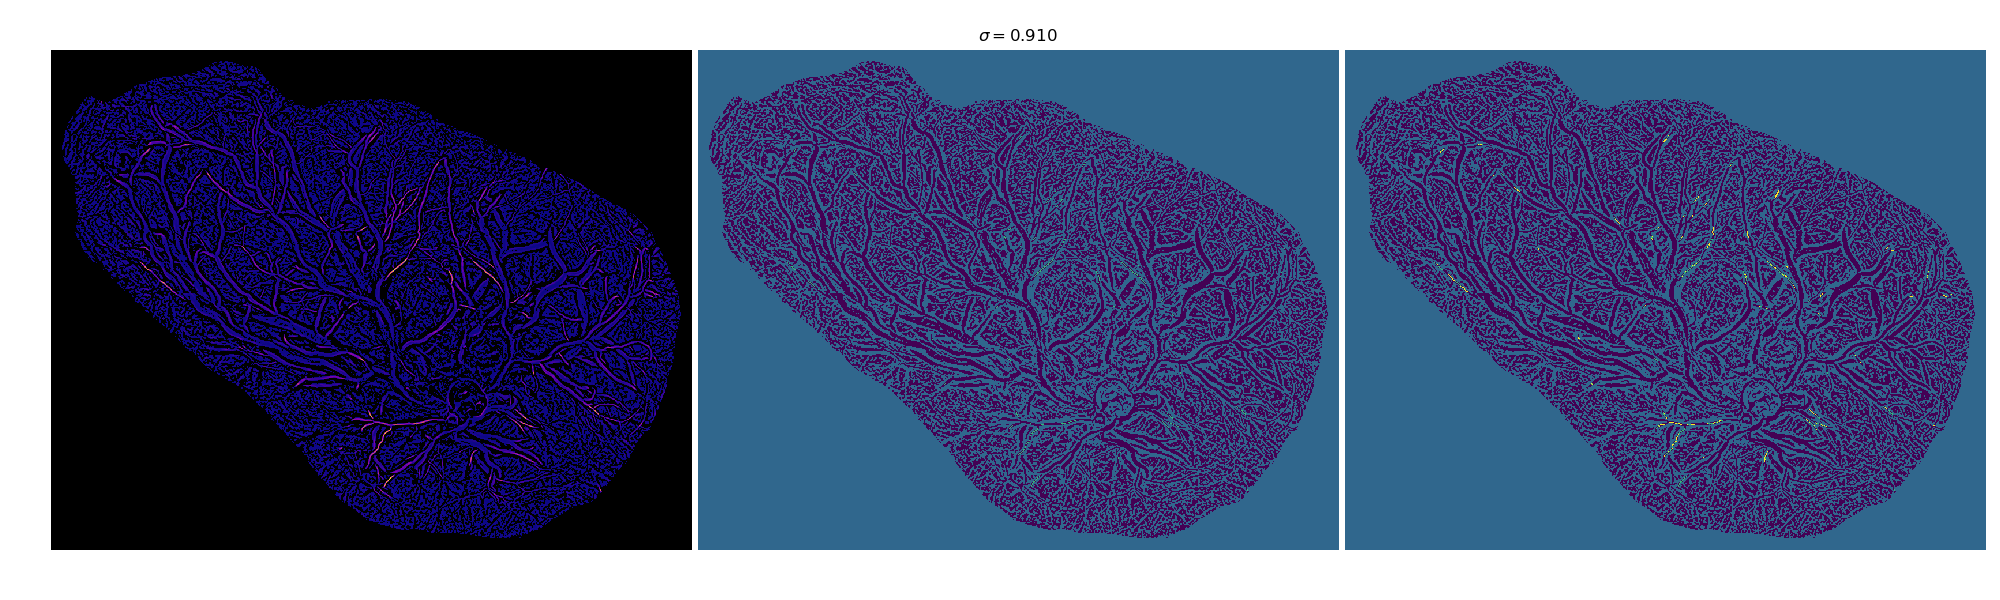
\includegraphics[width=\textwidth]{rw_demo_scale_03}
}\\[-0.5cm]
  \subfloat{
  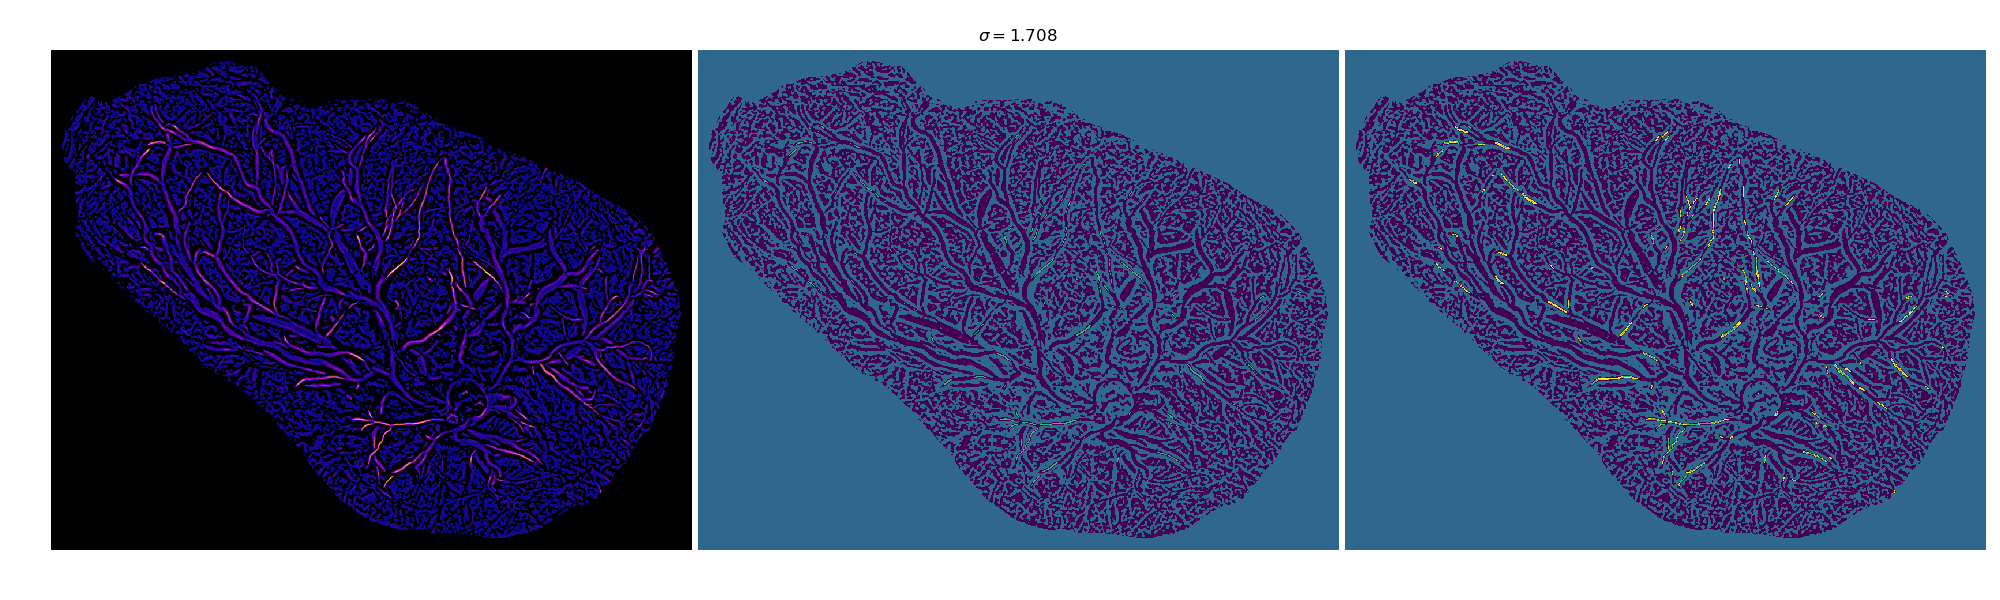
\includegraphics[width=\textwidth]{rw_demo_scale_05}
}\\[-0.5cm]
  \subfloat{
  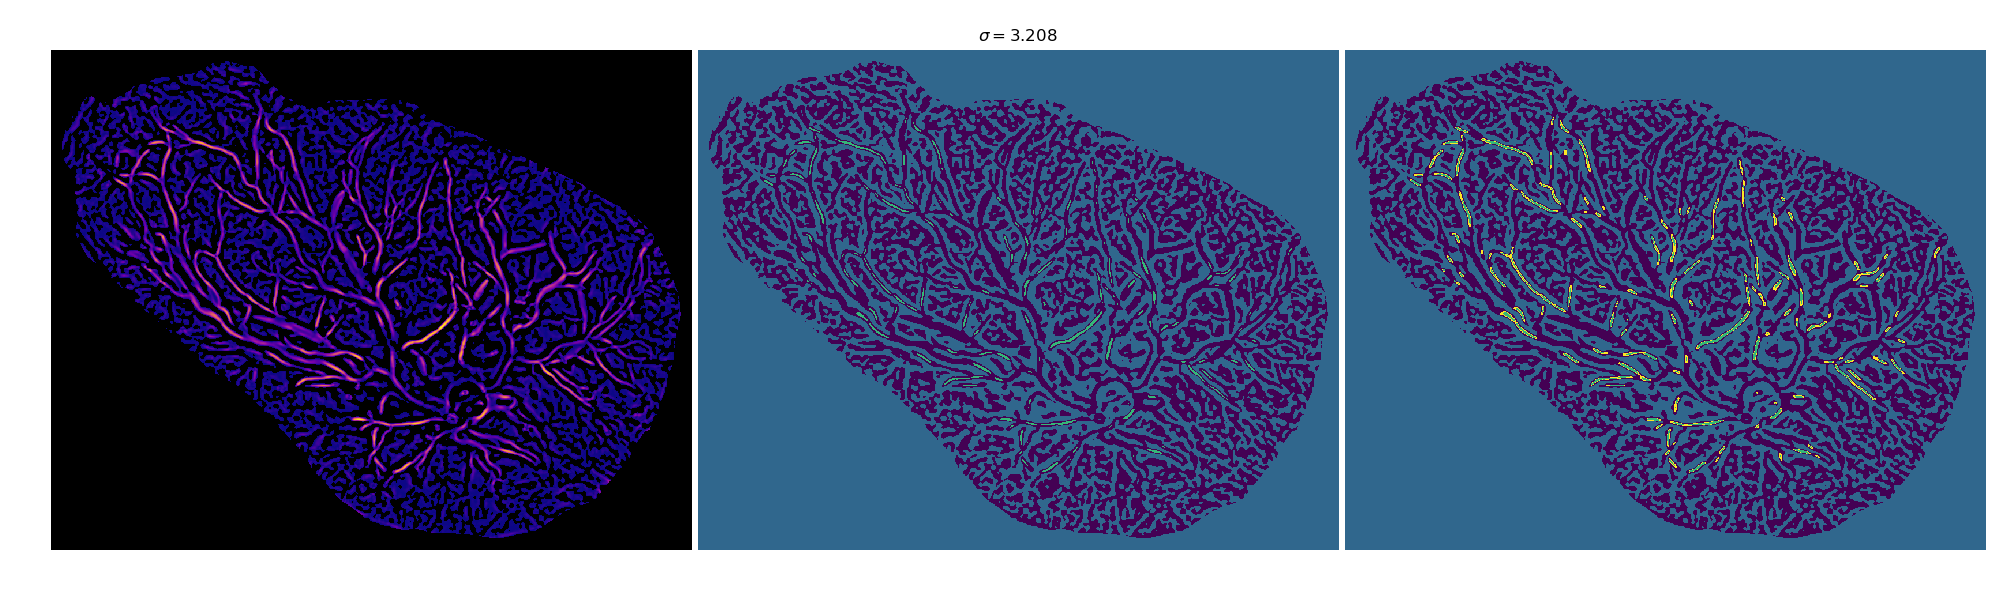
\includegraphics[width=\textwidth]{rw_demo_scale_07}
}\\[-0.5cm]
  \subfloat{
  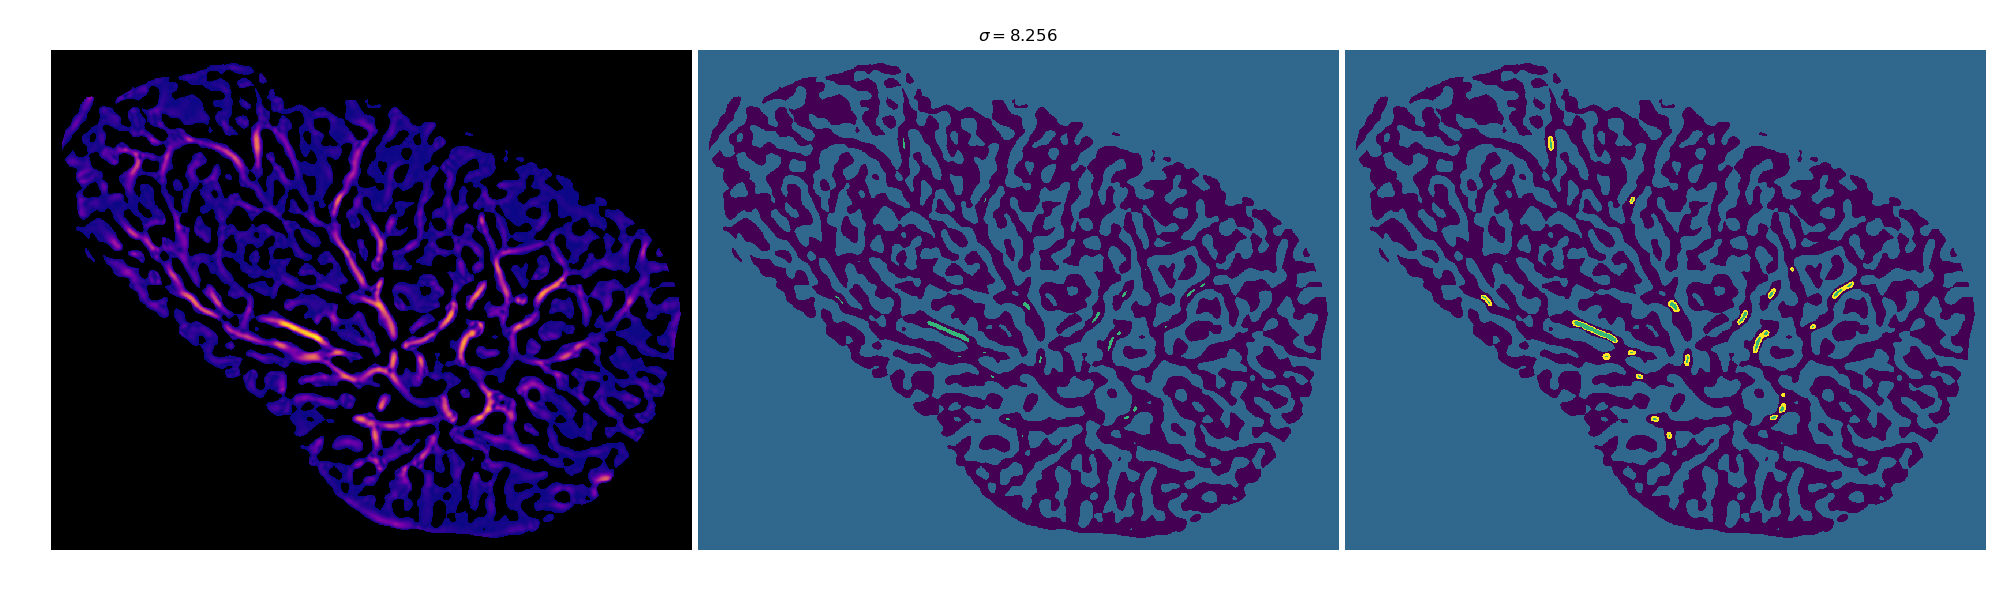
\includegraphics[width=\textwidth]{rw_demo_scale_10}
}
\caption{Scale-wise random walker segmentation (select scales)}
  \label{fig:rw-demo-scalewise}
\end{figure}
 
 
\begin{figure} \centering
  \subfloat{
    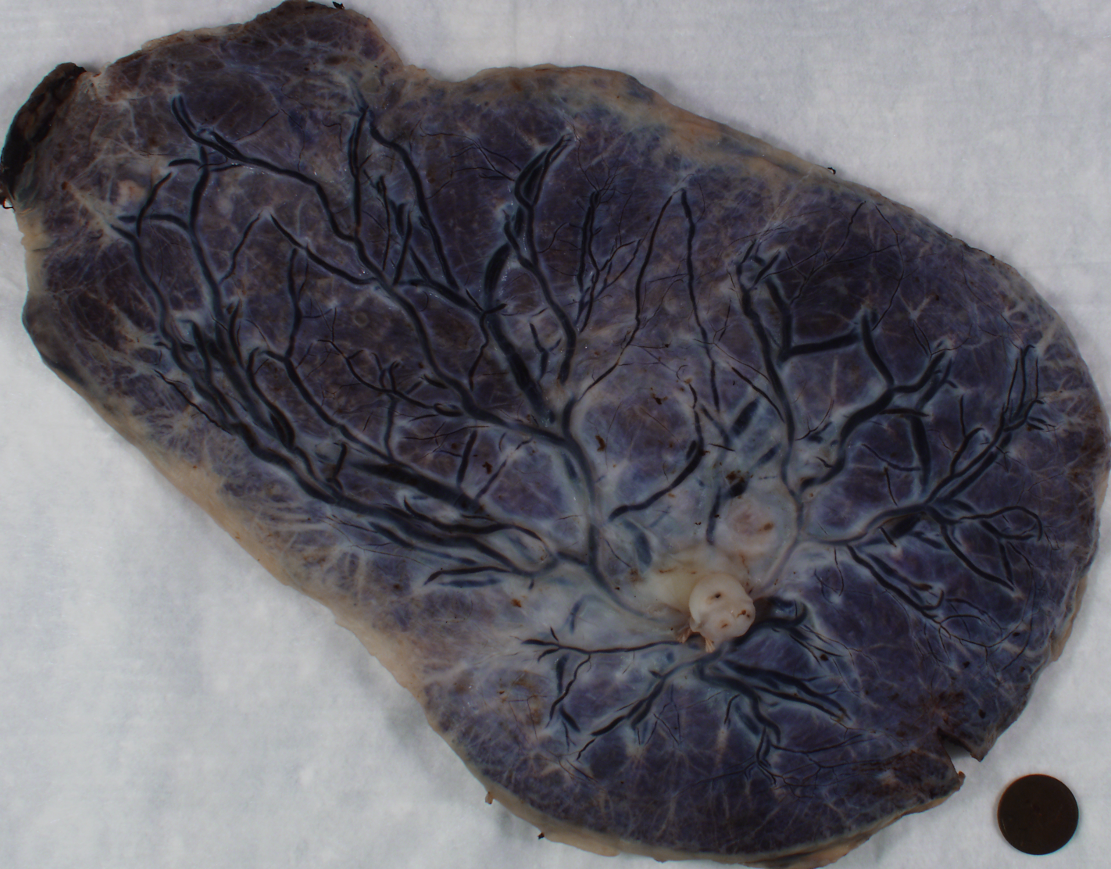
\includegraphics[height=0.4\textheight]{rw_demo_base}
  }\\[-0.5cm]
\subfloat{
    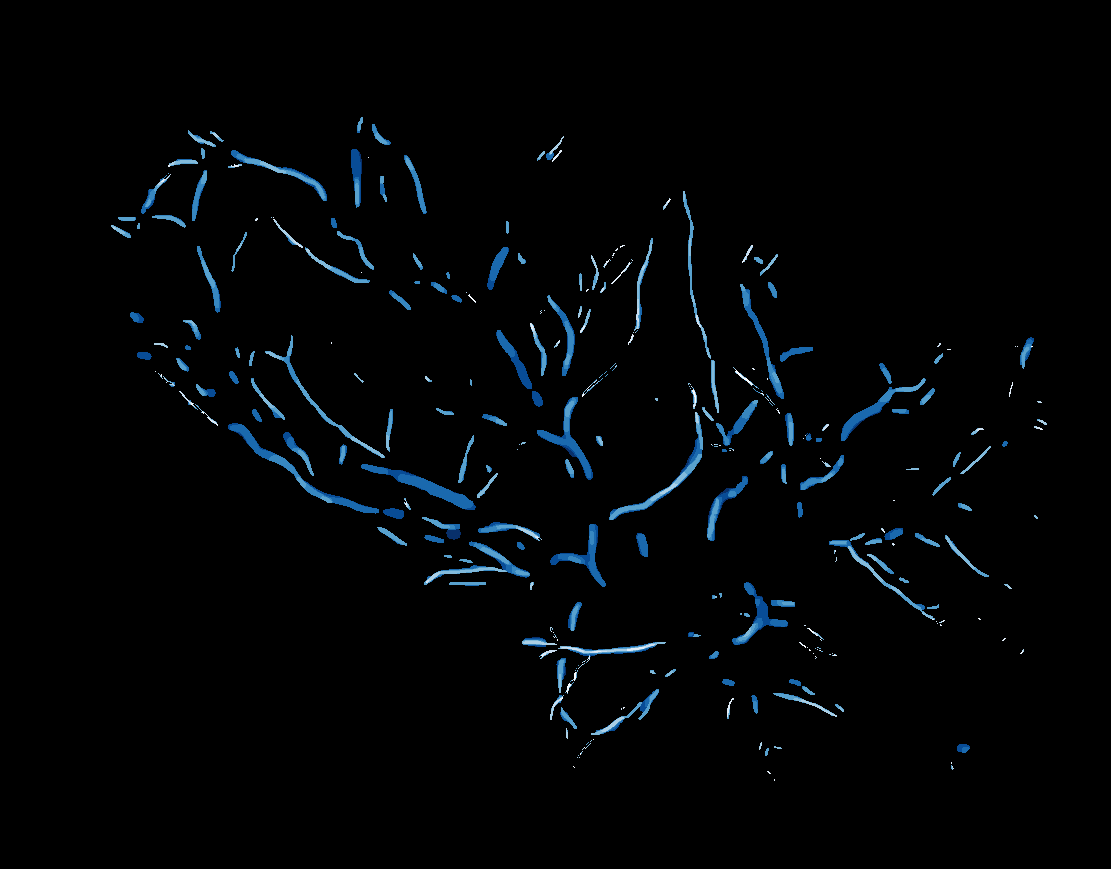
\includegraphics[height=0.4\textheight]{rw_demo_labels}
  }
  \caption{Random walker segmentation (result and sample)}
  \label{fig:rw-demo-merged}
\end{figure}

 \subsection{Method D: Scale Based Sieving}
   
  Our final approach seeks to include not only pixels at each scale that pass a high threshold, but also adjacent pixels at that scale that pass a lower threshold. We proceed as follows. At each scale, take a low threshold, then label each connected region. Then, iterate through each labeled region and add to the final approximation any labeled region that contains a pixel that passes a higher threshold.